\documentclass[12]{article}
\usepackage{array}
\usepackage{amsmath}
\usepackage{tabularx}
\usepackage{multicol,multirow}
\usepackage{enumitem}
\usepackage{graphicx}
\usepackage{subcaption} % for subfigures
\usepackage[a4paper, total={6.5in, 9.5in}]{geometry}

% Source : https://tex.stackexchange.com/questions/140567/drawing-karnaughs-maps-in-latex

%isolated term
%#1 - Optional. Space between node and grouping line. Default=0
%#2 - node
%#3 - filling color
\newcommand{\implicantsol}[3][0]{
    \draw[rounded corners=3pt, fill=#3, opacity=0.3] ($(#2.north west)+(135:#1)$) rectangle ($(#2.south east)+(-45:#1)$);
    }


%internal group
%#1 - Optional. Space between node and grouping line. Default=0
%#2 - top left node
%#3 - bottom right node
%#4 - filling color
\newcommand{\implicant}[4][0]{
    \draw[rounded corners=3pt, fill=#4, opacity=0.3] ($(#2.north west)+(135:#1)$) rectangle ($(#3.south east)+(-45:#1)$);
    }

%group lateral borders
%#1 - Optional. Space between node and grouping line. Default=0
%#2 - top left node
%#3 - bottom right node
%#4 - filling color
\newcommand{\implicantcostats}[4][0]{
    \draw[rounded corners=3pt, fill=#4, opacity=0.3] ($(rf.east |- #2.north)+(90:#1)$)-| ($(#2.east)+(0:#1)$) |- ($(rf.east |- #3.south)+(-90:#1)$);
    \draw[rounded corners=3pt, fill=#4, opacity=0.3] ($(cf.west |- #2.north)+(90:#1)$) -| ($(#3.west)+(180:#1)$) |- ($(cf.west |- #3.south)+(-90:#1)$);
}

%group top-bottom borders
%#1 - Optional. Space between node and grouping line. Default=0
%#2 - top left node
%#3 - bottom right node
%#4 - filling color
\newcommand{\implicantdaltbaix}[4][0]{
    \draw[rounded corners=3pt, fill=#4, opacity=0.3] ($(cf.south -| #2.west)+(180:#1)$) |- ($(#2.south)+(-90:#1)$) -| ($(cf.south -| #3.east)+(0:#1)$);
    \draw[rounded corners=3pt, fill=#4, opacity=0.3] ($(rf.north -| #2.west)+(180:#1)$) |- ($(#3.north)+(90:#1)$) -| ($(rf.north -| #3.east)+(0:#1)$);
}

%group corners
%#1 - Optional. Space between node and grouping line. Default=0
%#2 - filling color
\newcommand{\implicantcantons}[2][0]{
    \draw[rounded corners=3pt, opacity=.3] ($(rf.east |- 0.south)+(-90:#1)$) -| ($(0.east |- cf.south)+(0:#1)$);
    \draw[rounded corners=3pt, opacity=.3] ($(rf.east |- 8.north)+(90:#1)$) -| ($(8.east |- rf.north)+(0:#1)$);
    \draw[rounded corners=3pt, opacity=.3] ($(cf.west |- 2.south)+(-90:#1)$) -| ($(2.west |- cf.south)+(180:#1)$);
    \draw[rounded corners=3pt, opacity=.3] ($(cf.west |- 10.north)+(90:#1)$) -| ($(10.west |- rf.north)+(180:#1)$);
    \fill[rounded corners=3pt, fill=#2, opacity=.3] ($(rf.east |- 0.south)+(-90:#1)$) -|  ($(0.east |- cf.south)+(0:#1)$) [sharp corners] ($(rf.east |- 0.south)+(-90:#1)$) |-  ($(0.east |- cf.south)+(0:#1)$) ;
    \fill[rounded corners=3pt, fill=#2, opacity=.3] ($(rf.east |- 8.north)+(90:#1)$) -| ($(8.east |- rf.north)+(0:#1)$) [sharp corners] ($(rf.east |- 8.north)+(90:#1)$) |- ($(8.east |- rf.north)+(0:#1)$) ;
    \fill[rounded corners=3pt, fill=#2, opacity=.3] ($(cf.west |- 2.south)+(-90:#1)$) -| ($(2.west |- cf.south)+(180:#1)$) [sharp corners]($(cf.west |- 2.south)+(-90:#1)$) |- ($(2.west |- cf.south)+(180:#1)$) ;
    \fill[rounded corners=3pt, fill=#2, opacity=.3] ($(cf.west |- 10.north)+(90:#1)$) -| ($(10.west |- rf.north)+(180:#1)$) [sharp corners] ($(cf.west |- 10.north)+(90:#1)$) |- ($(10.west |- rf.north)+(180:#1)$) ;
}

%Empty Karnaugh map 4x4
\newenvironment{Karnaugh}%
{
\begin{tikzpicture}[baseline=(current bounding box.north),scale=0.8]
\draw (0,0) grid (4,4);
\draw (0,4) -- node [pos=0.7,above right,anchor=south west] {RS} node [pos=0.7,below left,anchor=north east] {PG} ++(135:1);
%
\matrix (mapa) [matrix of nodes,
        column sep={0.8cm,between origins},
        row sep={0.8cm,between origins},
        every node/.style={minimum size=0.3mm},
        anchor=8.center,
        ampersand replacement=\&] at (0.5,0.5)
{
                       \& |(c00)| 00         \& |(c01)| 01         \& |(c11)| 11         \& |(c10)| 10         \& |(cf)| \phantom{00} \\
|(r00)| 00             \& |(0)|  \phantom{0} \& |(1)|  \phantom{0} \& |(3)|  \phantom{0} \& |(2)|  \phantom{0} \&                     \\
|(r01)| 01             \& |(4)|  \phantom{0} \& |(5)|  \phantom{0} \& |(7)|  \phantom{0} \& |(6)|  \phantom{0} \&                     \\
|(r11)| 11             \& |(12)| \phantom{0} \& |(13)| \phantom{0} \& |(15)| \phantom{0} \& |(14)| \phantom{0} \&                     \\
|(r10)| 10             \& |(8)|  \phantom{0} \& |(9)|  \phantom{0} \& |(11)| \phantom{0} \& |(10)| \phantom{0} \&                     \\
|(rf) | \phantom{00}   \&                    \&                    \&                    \&                    \&                     \\
};
}%
{
\end{tikzpicture}
}

%Empty Karnaugh map 2x4
\newenvironment{Karnaughvuit}%
{
\begin{tikzpicture}[baseline=(current bounding box.north),scale=0.8]
\draw (0,0) grid (4,2);
\draw (0,2) -- node [pos=1.3,above right,anchor=south west] {$cs_{1}$,$cs_{0}$} node [pos=0.7,below left,anchor=north east] {$cs_{2}$} ++(135:1);
%
\matrix (mapa) [matrix of nodes,
        column sep={0.8cm,between origins},
        row sep={0.8cm,between origins},
        every node/.style={minimum size=0.3mm},
        anchor=4.center,
        ampersand replacement=\&] at (0.5,0.5)
{
                      \& |(c00)| 00         \& |(c01)| 01         \& |(c11)| 11         \& |(c10)| 10         \& |(cf)| \phantom{00} \\
|(r00)| 0             \& |(0)|  \phantom{0} \& |(1)|  \phantom{0} \& |(3)|  \phantom{0} \& |(2)|  \phantom{0} \&                     \\
|(r01)| 1             \& |(4)|  \phantom{0} \& |(5)|  \phantom{0} \& |(7)|  \phantom{0} \& |(6)|  \phantom{0} \&                     \\
|(rf) | \phantom{00}  \&                    \&                    \&                    \&                    \&                     \\
};
}%
{
\end{tikzpicture}
}

%Empty Karnaugh map 2x2
\newenvironment{Karnaughquatre}%
{
\begin{tikzpicture}[baseline=(current bounding box.north),scale=0.8]
\draw (0,0) grid (2,2);
\draw (0,2) -- node [pos=0.7,above right,anchor=south west] {b} node [pos=0.7,below left,anchor=north east] {a} ++(135:1);
%
\matrix (mapa) [matrix of nodes,
        column sep={0.8cm,between origins},
        row sep={0.8cm,between origins},
        every node/.style={minimum size=0.3mm},
        anchor=2.center,
        ampersand replacement=\&] at (0.5,0.5)
{
          \& |(c00)| 0          \& |(c01)| 1  \\
|(r00)| 0 \& |(0)|  \phantom{0} \& |(1)|  \phantom{0} \\
|(r01)| 1 \& |(2)|  \phantom{0} \& |(3)|  \phantom{0} \\
};
}%
{
\end{tikzpicture}
}

%Defines 8 or 16 values (0,1,X)
\newcommand{\contingut}[1]{%
\foreach \x [count=\xi from 0]  in {#1}
     \path (\xi) node {\x};
}

%Places 1 in listed positions
\newcommand{\minterms}[1]{%
    \foreach \x in {#1}
        \path (\x) node {1};
}

%Places 0 in listed positions
\newcommand{\maxterms}[1]{%
    \foreach \x in {#1}
        \path (\x) node {0};
}

%Places X in listed positions
\newcommand{\indeterminats}[1]{%
    \foreach \x in {#1}
        \path (\x) node {X};
}
\graphicspath{ {./Util/} }

\title{
\vspace{10mm}\\
CSE 306\\
Computer Architecture Sessional\\
\vspace{10mm}\\
Assignment-3: 4-bit MIPS Design, Simulation, and Implementation\\
\vspace{15mm}\\
Lab Section - A1\\
Group - 06\\
\vspace{5mm}\\
\large{11 February, 2024}\\
\vspace{20mm}
\raggedright
\Large{Members of the Group:\par}
\Large{
\begin{enumerate}[label = \roman*.]
    \item 2005020 - Mostafa Rifat Tazwar
    \item 2005025 - Most. Sonia Khatun
    \item 2005027 - Swastika Pandit
    \item 2005029 - MD. Minhajul Islam Fuad
    \item 2005030 - Fairuz Mubashwera
\end{enumerate}
}
}

\author{}
\date{}

\begin{document}

\maketitle
\newpage

\section{Introduction}
MIPS (Microprocessor without Interlocked Pipeline Stages) is a reduced instruction set computer (RISC) instruction set architecture (ISA) developed by MIPS Technologies. Instructions of MIPS are fixed, thus ensuring regularity.\\ Here is an example of sub instruction\\
\\
\begin{tabular}{|c|c|c|}
\hline
   Operation  & Instruction & Action  \\
   \hline
    Subtraction & sub \$t0, \$t1, \$t2 & \$t0 = \$t1 - \$t2\\
    \hline
\end{tabular}\\
\\
\\
Here \$t1, \$t2, \$t3 are registers that hold values. To evaluate an expression p = a-b–c,
we would do the following.\\
sub \$t0, \$t1, \$t2 [p = a-b]\\
sub \$t0, \$t0, \$t3 [p = p-c or p = a-b-c]
\\\\The prime objective of this assignment was to design an 4-bit processor which implements the MIPS instruction set.It took 1 clock cycle to execute each instruction. The length of the clock 
cycle was long enough so that the longest instruction on the MIPS instruction set was executed 
in a single clock cycle. Instruction memory, Data memory, Register file, ALU, Control unit were 
the main components of the processor. These components were designed and properly connected 
using some available multiplexers, adders and wires.

\section{Instruction Set}

\begin{table}[!h]
    \centering
\begin{tabular}{|c|c|c|c|c|}
\hline
Decimal (Opcode) & Instruction ID  & Category  & Type & Instruction \\
\hline
0(0000) & E & Logic & R & and \\
\hline
1(0001) & F & Logic & I & andi \\
\hline
2(0010)& N & Control-conditional & I & beq\\
\hline
3(0011) & P & Control-unconditional & J &  j \\
\hline
4(0100) & O & Control-conditional & I & bneq\\
\hline
5(0101) & C & Arithmetic & R & sub \\
\hline
6(0110) & D & Arithmetic & I & subi\\
\hline
7(0111) & B & Arithmetic & I & addi\\
\hline
8(1000) & I &  Logic & S & sll\\
\hline
9(1001) & G &  Logic & R & or\\
\hline
10(1010) & A & Arithmetic & R & add\\
\hline
11(1011) & H & Logic & I & ori \\
\hline
12(1100) & M & Memory & I & lw\\
\hline
13(1101) & J & Logic & S & srl \\
\hline
14(1110) & K & Logic & R & nor \\
\hline
15(1111) & L & Memory & I & sw \\
\hline

\end{tabular}
    \caption{Instruction set}
    \label{tab:ins_set}
\end{table}

\\



\section{Description Of Modules}
\subsection{Instruction Memory with Program Count}
Instruction Memory is the starting fundamental component of our MIPS. The instruction memory circuit takes an 8-bit program count (PC) and gives 16-bit instruction for the PC. Program Count is calculated using 8-bit binary adders. A ROM is used to store all possible 256 instructions and the circuit fetches the intended instruction for a particular program count. The instruction (output) is then split into 4-bit nibbles, for example, instruction bits [15:12] mean Opcode.There is a MUX in the circuit to select which 4-bit nibble will be used as the address for the destination register, and the MUX is controlled by RegDst control bit which comes from Control Unit. The circuit works in synchronization with clock signals.

\subsection{Data Memory With Stack}
Data Memory is the part of circuit that is used when we want to load word from memory element or store word in memory element. As input we give the 4 bit ALU output and 4 bit reg data which is to be written on a particular memory when we give store word command. A RAM is used as memory element as there will be frequent read and write operation on this memory. So there are also three control inputs which will come from the control unit. If memRead is 1, then the data from the given memory address will be given as output.If memWrite is 1, then the data will be written in given memory address. There is also a MUX to select whether the output of the ALU (for R-format) or the output of Data memory(for S format) will finally go as an output. MemToReg is the selection bit for this mux. If it is 1, output of the Data memory is selected and then the output goes to the register for write.The memory element also serves as the stack, where initially the end address of the memory signifies the top of the stack and the stack pointer handles the relevant operations.


\subsection{ALU}
An Arithmetic Logic Unit (ALU) is a fundamental component of a computer's central processing unit (CPU). It's responsible for performing arithmetic and bitwise logical operations on input data from registers or memory. In this assignment , the circuit takes two operands which are 4 bit number and an opcode which decides what type of operation is done by the ALU. After performing operation , the circuit produces a 4 bit output. 

\begin{table}[!h]
    \centering
    \begin{tabular}{|c|c|}
\hline
Opcode & Function \\
\hline
000 & ADD \\
\hline
001 & SUB \\
\hline
010 & OR \\
\hline
011 & AND \\
\hline
100 & NOR \\
\hline
101 & SLL \\
\hline
110 & SRL \\
\hline
\end{tabular}
    \caption{ALU Opcode}
    \label{tab:my_label}
\end{table}

\subsection{Register File}
\large
	This circuit takes as input two register addresses, ReadReg1 and ReadReg2 and outputs the associated data in those addresses of register file, namely ReadData1 and ReadData2.\\
	For write operation it takes four inputs, WriteData (the data to be written), WriteReg (the address of the register in which the data will be written), RegWriteEnable (whether this data should be written), and clock. WriteReg is input to a 3X8 decoder. When register x is selected, $RegSelect_{x}$ is 1. When $RegSelect_{x}$ is 1 and RegWriteEnable is 1, the given WriteData is input to that register, otherwise, the data previously stored in that register, $Q_n$ is input to that register. $$ Q_{x(n + 1)} = WriteEnable.RegSelect_x.WriteData + \overline{WriteEnable.RegSelect_x}.Q_{x(n)}$$

\newpage

\subsection{Control Unit}
\large
The control unit takes 4 bit Opcode as input and sets the relevant control bits for \textit{R, S, I and J-type} instructions according to the following table.


\begin{table}[!h]
    \centering
    \small
    \begin{tabular}{|c|c|c|c|c|c|c|c|c|c|c|c|c|}
        \hline
        \multirow{2}{*}{\textbf{Ins}} & \multirow{2}{*}{\textbf{Opcode}} & \multirow{2}{*}{\textbf{ALUOp}} & \multirow{2}{*}{\textbf{Branch}} & \multirow{2}{*}{\textbf{Jump}} & \multirow{2}{*}{\textbf{Bneq}} & \textbf{Mem} & \textbf{Mem} & \textbf{Mem} & \textbf{Reg} & Reg & ALU \\
        & & & & & & to Reg & Read & Write & Write & Dst & Src \\ \hline \hline
        PORTS & D$_3$D$_2$D$_1$D$_0$ & A$_7$A$_6$A$_5$ & A$_4$ & A$_3$ & A$_2$ & A$_1$ & A$_0$ & D$_7$ & D$_6$ & D$_5$ & D$_4$ \\ \hline
        and & 0000 & 011 & 0 & 0 & 0 & 0 & 0 & 0 & 1 & 1 & 0  \\ \hline
        andi & 0001 & 011 & 0 & 0 & 0 & 0 & 0 & 0 & 1 & 0 & 1 \\ \hline
        beq & 0010 & 001 & 1 & 0 & 0 & 0 & 0 & 0 & 0 & 0 & 0 \\ \hline
        j & 0011 & 111 & 0 & 1 & 0 & 0 & 0 & 0 & 0 & 0 & 0 \\ \hline
        bneq & 0100 & 001 & 1 & 0 & 1 & 0 & 0 & 0 & 0 & 0 & 0 \\ \hline
        sub & 0101 & 001 & 0 & 0 & 0 & 0 & 0 & 0 & 1 & 1 & 0 \\ \hline
        subi & 0110 & 001 & 0 & 0 & 0 & 0 & 0 & 0 & 1 & 0 & 1 \\ \hline
        addi & 0111 & 000 & 0 & 0 & 0 & 0 & 0 & 0 & 1 & 0 & 1 \\ \hline
        sll & 1000 & 101 & 0 & 0 & 0 & 0 & 0 & 0 & 1 & 0 & 1 \\ \hline
        or & 1001 & 010 & 0 & 0 & 0 & 0 & 0 & 0 & 1 & 1 & 0  \\ \hline
        add & 1010 & 000 & 0 & 0 & 0 & 0 & 0 & 0 & 1 & 1  & 0 \\ \hline
        ori & 1011 & 010 & 0 & 0 & 0 & 0 & 0 & 0 & 1 & 0 & 1 \\ \hline
        lw & 1100 & 000 & 0 & 0 & 0 & 1 & 1 & 0 & 1 & 0 & 1 \\ \hline
        srl & 1101 & 110 & 0 & 0 & 0 & 0 & 0 & 0 & 1 & 0 & 1 \\ \hline
        nor & 1110 & 100  & 0 & 0 & 0 & 0 & 0 & 0 & 1 & 1 & 0 \\ \hline
        sw & 1111 & 000 & 0 & 0 & 0 & 0 & 0 & 1 & 0 & 0 & 1 \\ \hline
        \hline
    \end{tabular}
    \label{tab:1}
    \caption{Control Bits For Opcodes}
\end{table}

\begin{table}[!h]
    \centering
    \begin{tabular}{|c|c|}
        \hline
        \textbf{Opcode (Binary)} & \textbf{Control (Hex Codes)} \\
        \hline
        0000 & 0x606 \\ \hline
        0001 & 0x605 \\ \hline
        0010 & 0x300 \\ \hline
        0011 & 0xe80 \\ \hline
        0100 & 0x340 \\ \hline
        0101 & 0x206 \\ \hline
        0110 & 0x205 \\ \hline
        0111 & 0x005 \\ \hline
        1000 & 0xa05 \\ \hline
        1001 & 0x406 \\ \hline
        1010 & 0x006 \\ \hline
        1011 & 0x405 \\ \hline
        1100 & 0x035 \\ \hline
        1101 & 0xc05 \\ \hline
        1110 & 0x806 \\ \hline
        1111 & 0x009 \\ \hline
    \end{tabular}
    \caption{Hex Code of Control bits}
    \label{tab:2}
\end{table}

\newpage

\section{Circuit}
\subsection{Main Circuit:}
    
    \begin{figure}[!h]
        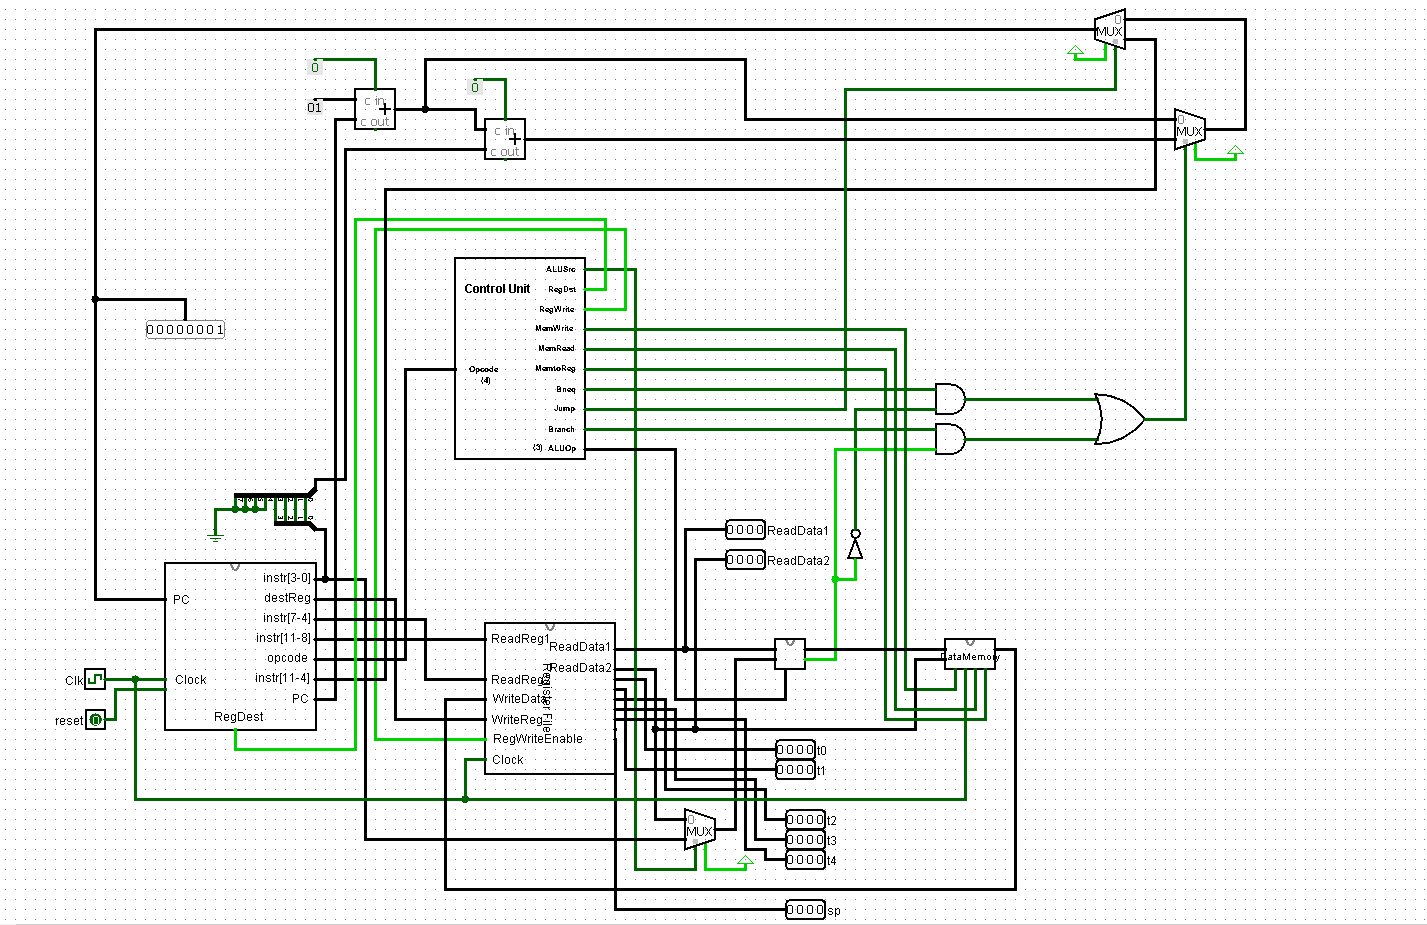
\includegraphics[scale = 0.5]{Images/Main circuit.png}
        \caption{\textbf{4 Bit MIPS Processor}}
    \end{figure}

\subsection{Detailed Circuit: }
    \begin{figure}[!h]
        \centering
        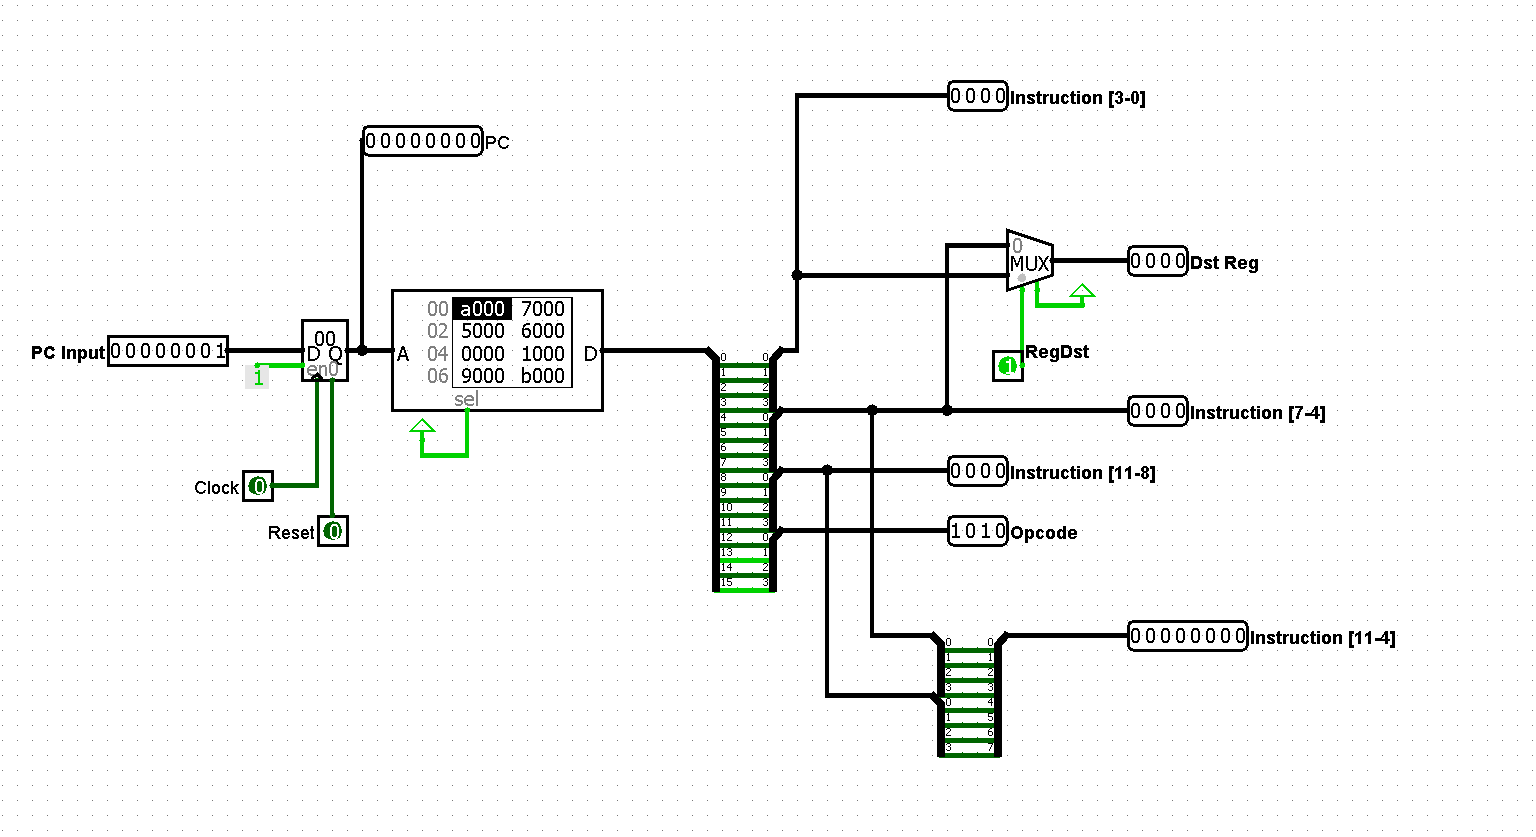
\includegraphics[scale = 0.45]{Images/Instruction Memory.png}
        \caption{\textbf{Instruction Memory}}
    \end{figure}

\begin{figure}[t]
    \centering
    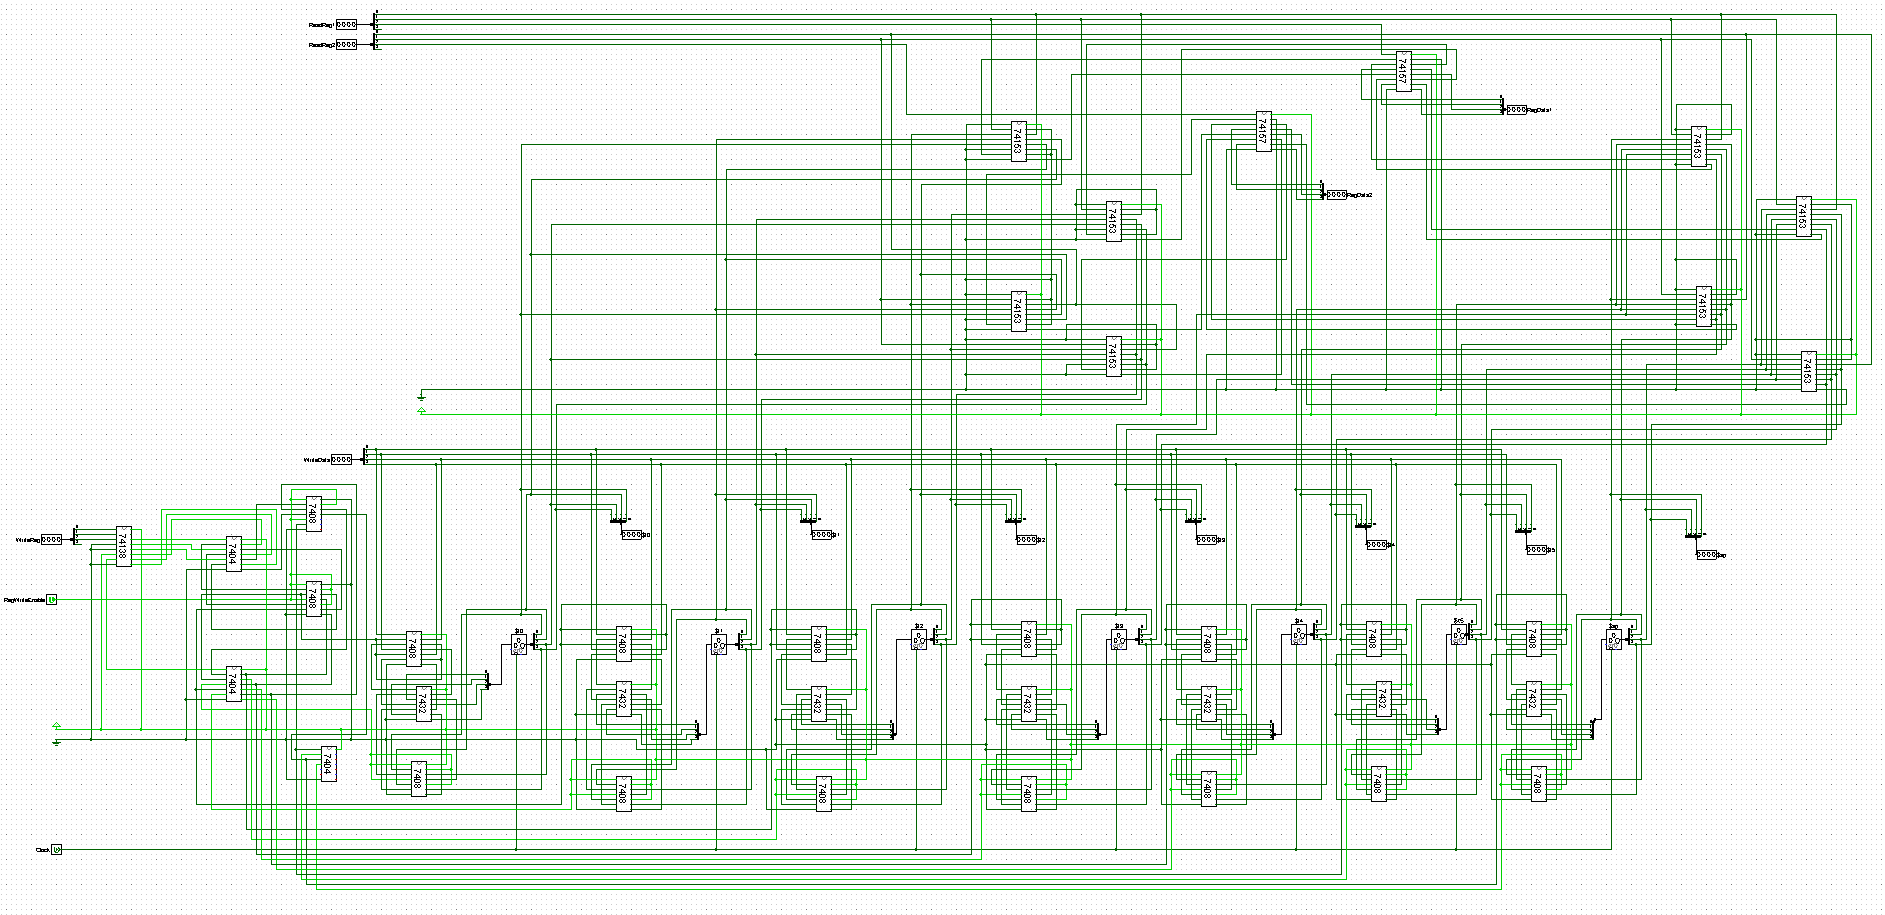
\includegraphics[scale = 0.4]{Images/Register File.png}
    \caption{\textbf{Register File}}
\end{figure}

\begin{figure}[!h]
    \centering
    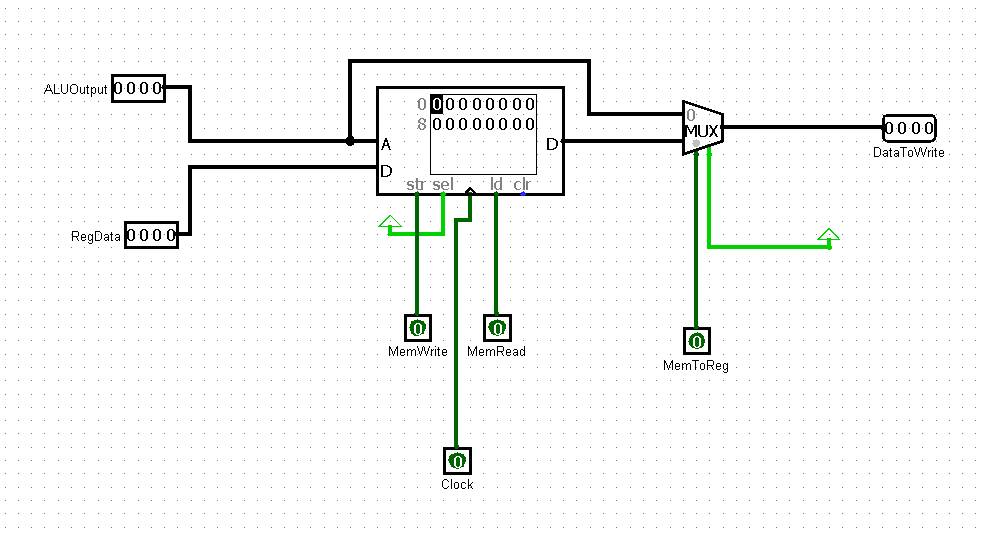
\includegraphics[scale = 0.75]{Images/Data Memory.png}
    \caption{\textbf{Data Memory}}
\end{figure}

\begin{figure}[b]
    \centering
    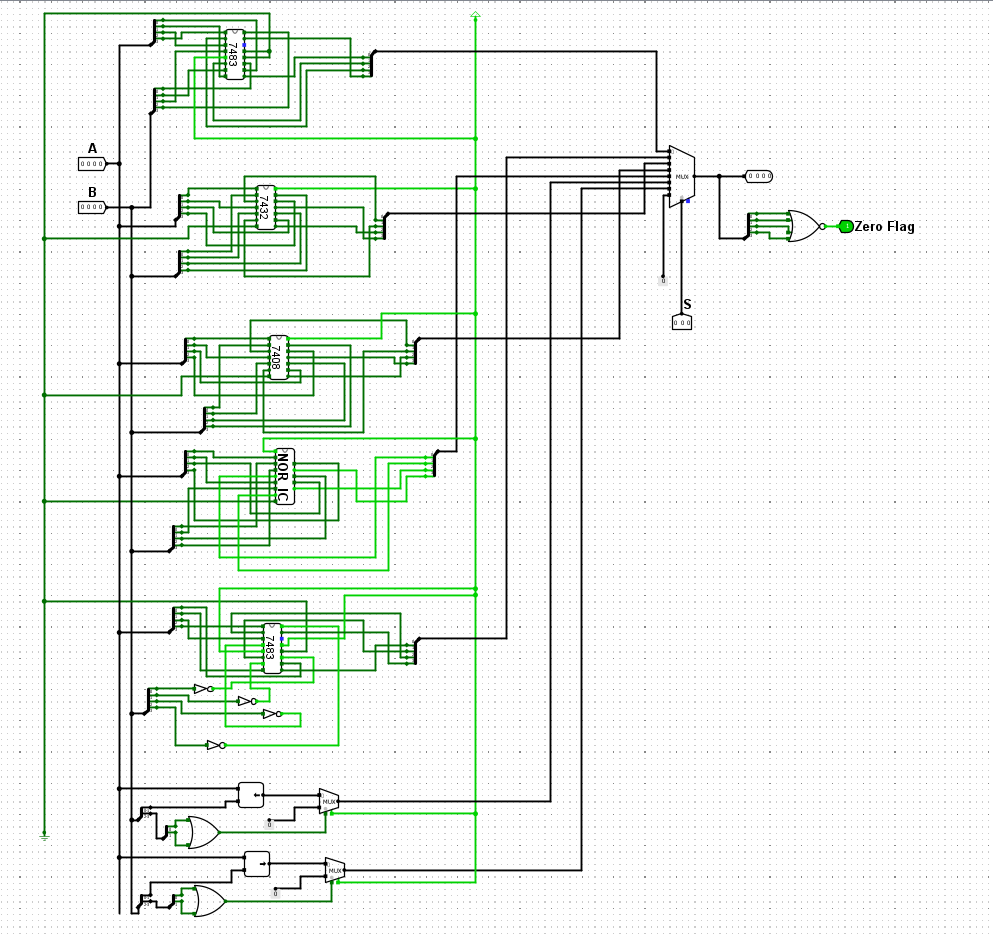
\includegraphics[scale = 0.75]{Images/ALU.png}
    \caption{\textbf{ALU}}
\end{figure}

\begin{figure}[t]
    \centering
    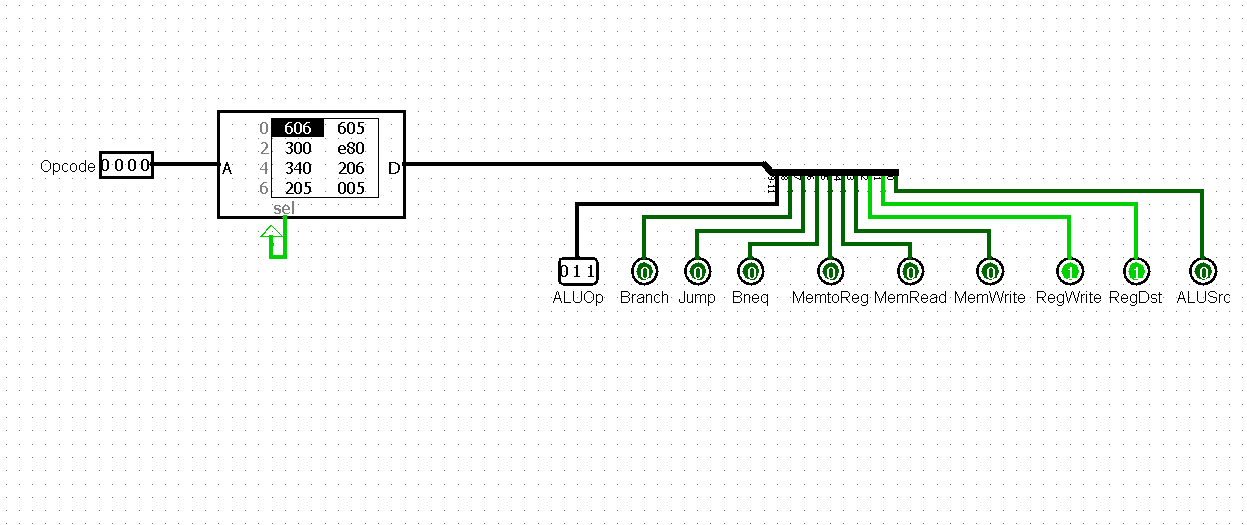
\includegraphics[scale = 0.6]{Images/Control Unit.png}
    \caption{\textbf{Control Unit}}
\end{figure}
\clearpage

\section{Approach to implement the push and pop instructions}

We maintained a stack memory in Data Memory Unit and a stack pointer in the register file. MIPS follows the RISC architecture. So, there were no direct instructions for push and pop. However, we used pseudo instructions to implement push, push offset, and pop instructions as follows:

\begin{table}[!h]
    \centering
    \begin{tabular}{|c|c|}
        \hline
        Instructions & Pseudo Instructions \\ 
        \hline
        \multirow{2}{*}{push \$t1} & sw \$t1, 0(\$sp) \\
         & subi \$sp, \$sp, 1 \\ 
         \hline
         \multirow{3}{*}{push 3(\$t1)} & lw \$t5, 3(\$t1) \\
        & sw \$t5, 0(\$sp) \\
        & subi \$sp, \$sp, 1 \\ 
        \hline 
        \multirow{2}{*}{pop \$t1} & addi \$sp, \$sp, 1 \\
        & lw \$t1, 0(\$sp) \\ 
        \hline
    \end{tabular}
    \caption{Pseudo Instructions For Push-Pop}
    \label{tab:3}
\end{table}

Although these instructions require 2, 3, and 2 clock cycles, respectively, there was no need for handling them separately.

\section{Approach to implement branch operation}

We had to implement beq and bneq operations in our design. For this, we used two control bits branch and bneq from the control unit. Whether branch is enabled or not is decided using the zero flag of the ALU unit.

\begin{table}[!h]
    \centering
    \begin{tabular}{|c|c|c|c|}
         \hline
        Branch & Bneq & Zero Flag & Branch Enable \\ \hline
         0 & x & x & 0 \\ \hline
         1 & 0 & 0 & 0 \\ \hline
         1 & 0 & 1 & 1 \\ \hline
         1 & 1 & 0 & 0 \\ \hline
         1 & 1 & 1 & 1 \\ \hline
         \hline
    \end{tabular}
    \caption{Branch Enable}
    \label{tab:BEN}
\end{table}
\raggedright
$Branch Enable = Branch \land ( Bneq \oplus Zero  )$


\section{IC Count}

\begin{table}[!h]
    \centering
    \begin{tabular}{| c | c |}
        \hline
        \textbf{IC} & \textbf{Count}\\  \hline \hline
        Atmega32 & 6 \\ \hline
        IC-7483 & 4 \\ \hline
        IC-74157 & 7 \\ \hline
    \end{tabular}
    \caption{IC Count for MIPS}
    \label{tab:count_table}
\end{table}

\section{The Simulator Used along with the Version Number}
\large
Logisim - 2.7.1


\section{Discussion}
\large
In this project, we implemented a 4 bit Mips supporting the instruction set as specified here \ref{tab:ins_set}. \\

We initially implemented the software simulation using \textbf{Logisim}. For simulating atmega32 we used Ram and Rom. In line with our hardware design, we also implemented a proteus design. For converting mips assembly to hex for instruction memory, we designed a compiler. It also generates the hex codes needed for the logisim design. We also implemented a manual clock and reset in our design.

The register file has 8 registers in total with 6 temporary registers (\$t0, \$t1,\$t2,\$t3,\$t4,\$t5), 1 zero register \$zero , and 1 
stack pointer register(\$sp) which is an extra temporary register was used to implement the push-pop instructions 
associated with memory.\\
From the ALU, we demonstrated output in each step of operation.
The value of PC was also shown for each clock cycle. All of our ATmega were tested before integrating it to our final circuit.Wires with different sizes were used to make the whole circuit organized and easily
understandable for the user.The outputs were checked multiple times for a large number of input test cases to
ensure that our circuit satisfies the expected output values.\\
Using minimal number of ICs in order to reduce complexity was the priority while designing the 
circuit. Outputs of some of the ICs were reused to minimize the circuit 
even more. The connections were made carefully and the components were placed at fair distances. 
Messiness was avoided as much as possible to ensure higher readability. Suitable labels were 
used at different parts of the circuit to make the functions of individual parts more 
understandable. Finally, the circuit was tested several times to make sure it did not have any sort 
of error.

\section{Contribution}
\subsection*{2005020 - Mostafa Rifat Tazwar}
\begin{itemize}
    \item Simulation
    \begin{itemize}
        \item Control Unit \& Bug fix
    \end{itemize}
    \item Report
    \begin{itemize}
        \item Control Unit
        \item Approach to implement the push,pop and branch instructions 
        \item IC Count
    \end{itemize}
\end{itemize}

\subsection*{2005025 - Most. Sonia Khatun}
    \begin{itemize}
        \item Simulation 
        \begin{itemize}
            \item ALU Unit
        \end{itemize}
        \item Report
        \begin{itemize}
            \item Introduction \& Instruction Set
            \item Discussion \& ALU
        \end{itemize}
    \end{itemize}

\subsection*{2005027 - Swastika Pandit}
\begin{itemize}
    \item Simulation
    \begin{itemize}
        \item Register File
        \item Connecting the components to form complete circuit
    \end{itemize}
    \item Report
    \begin{itemize}
        \item Register File
    \end{itemize}
    \item Hardware Implementation
\end{itemize}

\subsection*{2005029 - MD. Minhajul Islam Fuad}
\begin{itemize}
    \item Simulation
    \begin{itemize}
        \item Instruction Memory with PC
    \end{itemize}
    \item Report
    \begin{itemize}
        \item Circuit Diagram
        \item Instruction Memory with PC
    \end{itemize}    
\end{itemize}

\subsection*{2005030 - Fairuz Mubashwera}
\begin{itemize}
    \item Simulation
    \begin{itemize}
        \item Data Memory
    \end{itemize}
    \item Report
    \begin{itemize}
        \item Data Memory With Stack
    \end{itemize}
    \item Hardware Implementation
\end{itemize}

\end{document}
